%!TEX TS-program = xelatex

% HSE Beamer Theme
% by Danil Fedorovykh
% http://hse.ru/staff/df
%
% Version 2.0 (English)
% January 2022

%%% Set up the free HSE Sans font
%%% https://www.hse.ru/info/brandbook/#font

\documentclass[aspectratio=169]{beamer}

\newbool{russian}
%\booltrue{russian} % Uncomment if in Russian
\usepackage{HSE-theme/beamerthemeHSE} % Load HSE theme
\usepackage[inkscapeexe="/Applications/Inkscape.app/Contents/MacOS/inkscape", inkscapeopt=-z -D]{svg}

\usepackage[no-math]{fontspec}      % fonts loading
	\setsansfont{HSE Sans} 
	\setmonofont{Courier New}

\usepackage{blindtext} 		% Lorem ipsum
\usepackage{listings}
\graphicspath{{images/}}  	% Images folder

%%% Информация об авторе и выступлении
\title[Title]{Как отличить шум от хаотического временного ряда} 
\author[Author's name]{Presenter: Alexander Glushko}
\institute{Master's Programme Data Science}
\date{\today}


\begin{document}

\frame[plain]{\titlepage}

\begin{frame}
  \frametitle{Введение}
  \begin{itemize}
    \item Временные ряды можно разделить на:
    \begin{enumerate}
      \item хаотические;
      \item регулярные.
    \end{enumerate}
    \item Как разделить временные ряды и отличить их от шума?
  \end{itemize}
  \bigskip
  Rosso, Osvaldo \& Larrondo, Hilda \& Martin, M.T. \& Plastino, A. \& Fuentes, Miguel. (2007). Distinguishing Noise from Chaos. Physical review letters. 99. 154102. 10.1103/PhysRevLett.99.154102.
\end{frame}

\begin{frame}
  \frametitle{Мера сложности и энтропия Шеннона}
  \medskip

  Шенноновская энтропия: $S[P] = - \sum\limits^N_{j=1}p_j\ln(p_j)$
  
  \medskip 

  Мера на основе Шеноновской энтропии: $H_S[P] = \frac{S[P]}{S_max}$
  
  \bigskip 

  Сложность на основе дивергенция Дженсена-Шеннона: $$C_{JS}[P] = Q_J[P, P_e]H_S[P]$$
  
  \medskip

  Дивергенция Дженсена-Шеннона: $$Q_J[P, P_e] = Q_0 (S\left[ \frac{P + P_e}{2} \right] - \frac{S[P]}{2} - \frac{S[P_e]}{2})$$ 
\end{frame}

\begin{frame}
  \frametitle{Реализация}
  \medskip
  \begin{center}
    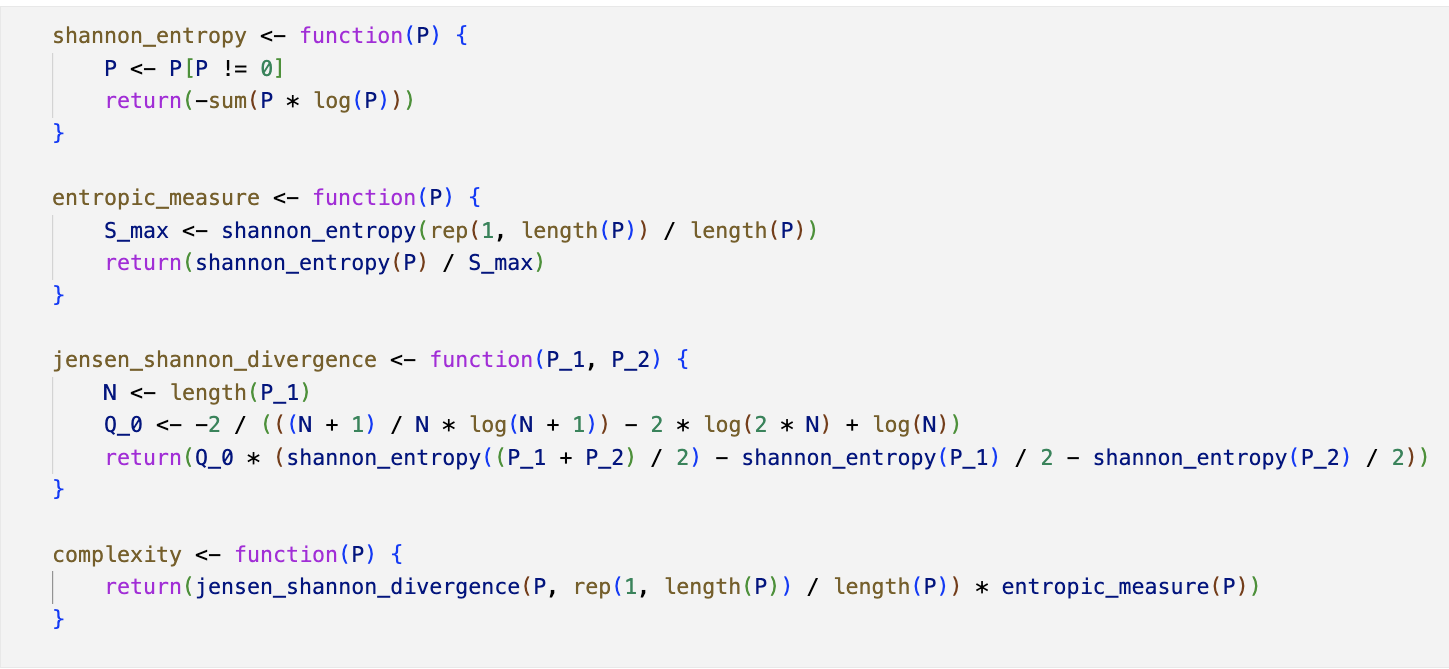
\includegraphics[width=0.85\columnwidth]{EntropyFunction.png}
  \end{center}
\end{frame}

\begin{frame}
  \frametitle{Максимальные и минимальные границы}
  \medskip
  \begin{center}
    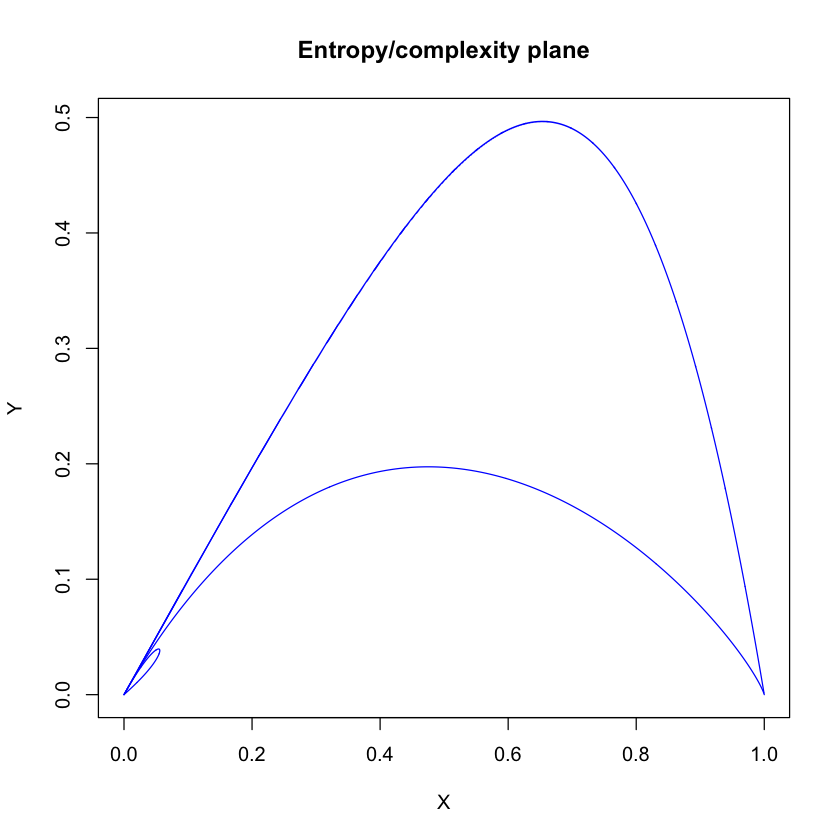
\includegraphics[width=0.5\columnwidth]{Plane.png}
  \end{center} 
\end{frame}

\begin{frame}
  \frametitle{Реализация}
  \medskip
  \begin{columns}
    \column{0.5\textwidth}
    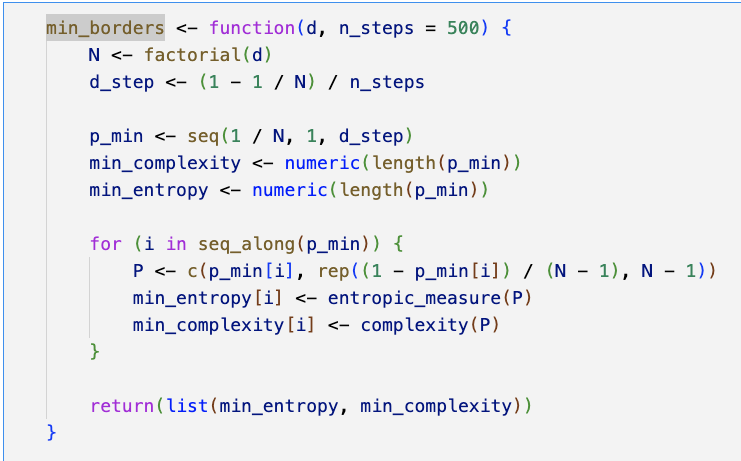
\includegraphics[width=\columnwidth]{min_border.png}
    
    \column{0.5\textwidth}
    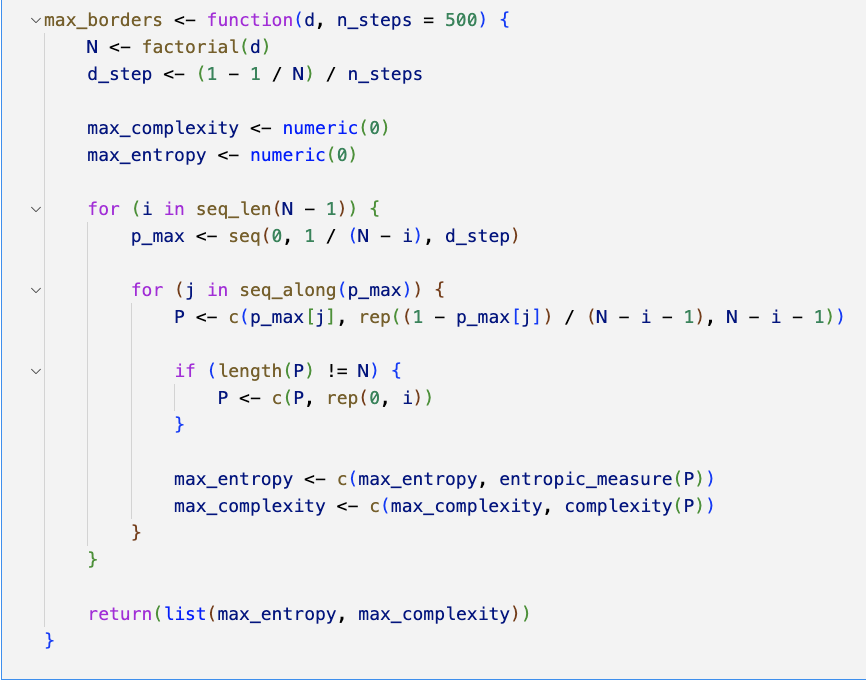
\includegraphics[width=\columnwidth]{max_border.png}
    \end{columns}
\end{frame}

\begin{frame}
  \frametitle{Преобразование временного ряда в вектор}
  \bigskip
  Для того чтобы получить вектор вероятностей из временного ряда воспользуемся порядковым шаблоном. 
  \medskip
  \begin{center}
    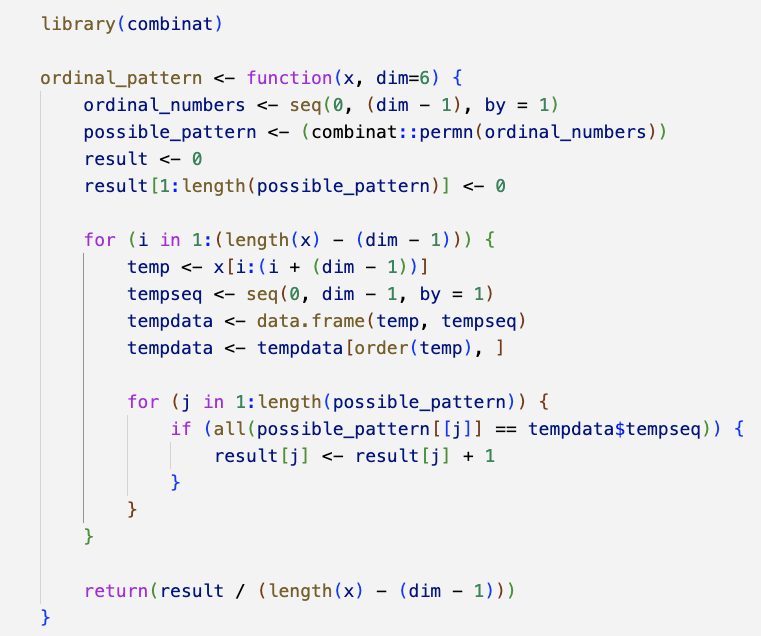
\includegraphics[width=0.5\columnwidth]{ordinal_pattern.png}
  \end{center}  
\end{frame}

\begin{frame}
  \frametitle{Временные ряды для тестирования}
  \begin{itemize}
    \item Хаотические:
    \begin{enumerate}
      \smallskip
      \item Skew tent map
      \smallskip
      \item Logistic map
      \smallskip
      \item Schuster's map
    \end{enumerate} 
    \medskip
    \item Гауссовский шум
    \medskip
    \item Значения синуса
  \end{itemize}
\end{frame}

\begin{frame}
  \frametitle{Итоговый график с точками рядов}
  \medskip
  \begin{center}
    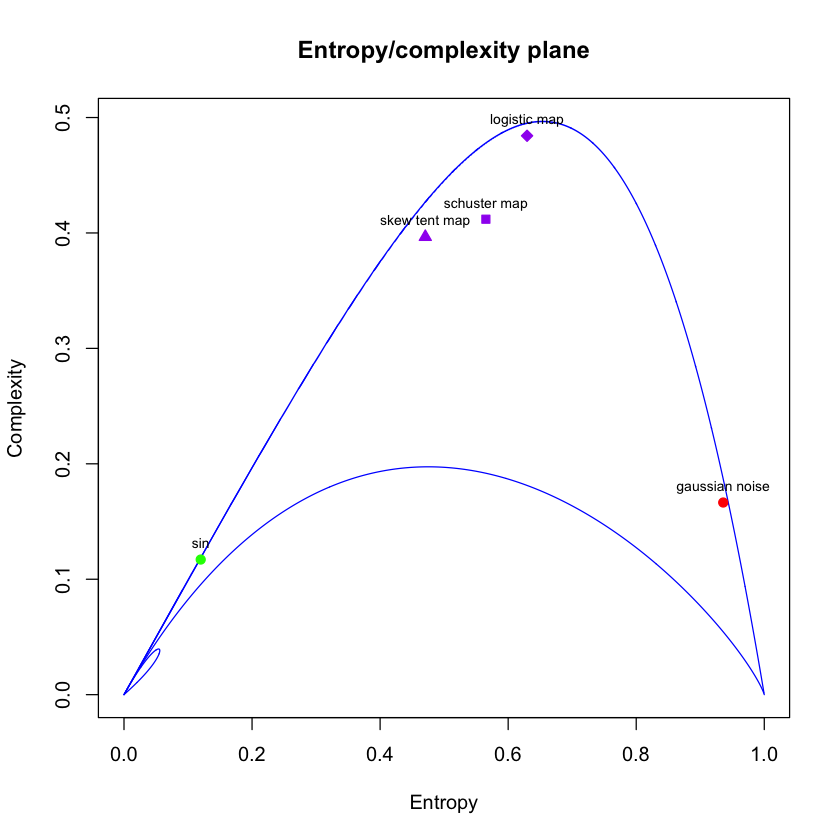
\includegraphics[width=0.5\columnwidth]{EntropyComplexityPlane.png}
  \end{center} 
\end{frame}

\begin{frame}
  \frametitle{Discussion}
  \bigskip
  \begin{center}
    \LARGE Thank you!
  \end{center}
  \vspace{80pt} 
  Repository with all code: \url{https://github.com/Kumokage/entropy_complexity_plane}
\end{frame}

\end{document}